%!TEX encoding = UTF-8 Unicode
%!TEX root = ../compendium2.tex

\Lab{\LabWeekTEN}

\begin{Goals}
\item Kunna använda mönstermatchning.
\item Kunna förklara hur \code{Option} användas för att hantera saknde värden.
\item Kunna använda \code{scala.util.Try} för att hantera undantag.
%\item Känna till att undantag kan hanteras med \code{try catch}.
%\item Kunna använda inbyggda sorteringsfunktioner \code{sortBy} och \code{sortWith}.
%\item Kunna implementera insättningssortering till ny sekvens.
\item Känna till hur strängar ordnas.
\item Kunna implementera registrering (frekvensräkning).
%\item Kunna använda matriser med strängar.
\end{Goals}

\begin{Preparations}
%\item \StudyTheory{12}
\item Gör övning {\texttt{\ExeWeekTEN}}, speciellt uppgift \ref{task:labprep-patterns-tabular}.
\item \ReadTheLab
\item Fyll i denna enkät: \url{https://goo.gl/forms/hC6JK2UQXVpbGECc2}  \\
I enkäten ska du för olika flervalsalternativlistor besvara frågan: \\ \textit{Vilket är ditt favoritalternativ?}
\item Studera den givna koden i \code{src/main/scala/tabular} här: \url{https://github.com/lunduniversity/introprog/tree/master/workspace/w10_tabular}
\end{Preparations}


\subsection{Bakgrund}

I den här veckans laboration ska du utveckla en terminalapplikation som analyserar data i tabeller. Indata utgörs av text med \textbf{kolumnseparerade värden}, där varje rad följs av \code{`\n`} och innehåller kolumner som är separerade med ett valfritt s.k. separator-tecken, till exempel \code{','}, \code{'\t'} eller \code{';'}. Din app ska förutsätta att första indataraden innehåller kolumnrubriker.

Du ska använda din app till att analysera svar på enkäter med flervalsfrågor, där varje persons svar finns på en egen rad och varje svarsrad innehåller svarsalternativ i kolumner.
Exempelindata finns i filen \code{favorit.csv} i mappen resources och ser ut som följer. Kolumnseparator i tabellen nedan är \code{","}. Första raden är en rubrikrad som anger kolumnernas respektive rubrik.
\lstinputlisting[basicstyle=\ttfamily\fontsize{10}{12}\selectfont]{../workspace/w10_tabular/src/main/resources/favorit.csv}

\subsection{Krav}

\begin{enumerate}[leftmargin=*]
\item Din applikation ska kunna behandla kolumndata i en tabell kallad \code{currentTable}.

\item Den aktuella tabellen ska kunna laddas från disk via filnamn eller från en webbadress som börjar med \code{http}.

\item Din applikation ska acceptera noll, ett eller två argument vid uppstart, där man kan styra ev. textkälla och ev. kolumnseparator.

\item Din applikation ska interagera med användaren genom terminalen och acceptera textkommandot \code{help} som ska ge följande utskrift. Körningen visar utskrift efter uppstart utan argument och resultatet av att användaren skrivit kommandot \code{help} efter prompten \code{"> "}.

\begin{REPLnonum}
Welcome to tabular: an app for analysis of data in tables
Current dir: /home/bjornr/pgk/labs/w10_tabular
No args given. Starting with empty table.
Type 'help' for help on commands and 'quit' to exit app.
> help
Commands:
help                 Print this list of commands
ls                   List files in current directory
load                 Load a file using introprog.Dialog.file
load filename|url    Load a table from <location> using current separator
save                 Save
save filename        Save current table to <filepath>
sep                  Show current column separator
sep c                Change current column separator to char c
show                 Print current table to the console
sort h               Sort current table on heading h
filter h a b c ...   Keep rows where heading h has values a b c ...
pie h                Draw a pie chart of current table's heading h
bar h                Draw a bar chart of current table's heading h
quit, Ctrl+D         Terminate app
\end{REPLnonum}
Följande kommandon är redan implementerade i given kod i modulen \code{Command}: \code{help}, \code{quit}, \code{Ctrl+D} och \code{ls}. Efter listorna nedan med obligatoriska och valfria krav finns en exempelkörning där utdata från olika kommando illustreras.

\item Du ska implementera följande \textbf{obligatoriska} funktioner:
\begin{itemize}[nosep, label={$\square$},]
\item \code{load filename|url} -- laddar \code{currentTable} från fil eller url
\item \code{show} -- visar tabellen i ett inramat rutnät i terminalen (se exempel)
\item \code{sep} -- visar aktuell kolumnseparator
\item \code{sep c} -- ändrar aktuell kolumnseparator till första tecknet i strängen \code{c}
\item \code{sort h} -- sorterar tabellens rader så att kolumnen med rubriken \code{h} är sorterad i bokstavsordning.
\item \code{filter h a b c ...} -- gör så att aktuell tabell bara innehåller de rader där kolumnen med rubriken \code{h} har något av angivna värdena \code{a b c ...}. Värdena ska var minst ett och separeras med blanktecken efter kolumnnamnet \code{h}.
\end{itemize}

\item Du ska implementera \emph{minst en} av följande \textbf{valfria} funktioner:
\begin{itemize}[nosep, label={$\square$},]
\item \code{load} -- laddar tabell från fil som anges av användaren i en filväljardialog med hjälp av \code{introprog.Dialog.file}
\item \code{save} -- sparar tabell som text till fil som anges av användaren i en filväljardialog med hjälp av \code{introprog.Dialog.file}
\item \code{pie h} -- ritar ett tårtdiagram över antalet förekomster av olika värden i kolumnen med rubriken \code{h} med hjälp av givna koden i \code{Graph.scala}.
\item \code{bar h} -- ritar ett stapeldiagram över antalet förekomster av olika värden i kolumnen med rubriken \code{h} med hjälp av givna koden i \code{Graph.scala}.
\item Implementera valfria funktioner för att göra beräkningar på \emph{numeriska} data i kolumner, t.ex. summa, medelvärde, standardavvikelse.
\end{itemize}

\end{enumerate}

\subsection{Design}

Du ska bygga vidare på den delvis färdiga koden i \code{workspace/w10_tabular} enligt denna design:
\begin{itemize}

\item Alla abstraktioner ska ligga i paketet \code{tabular}.

\item Den färdiga modulen \code{Main} hanterar ev. argument och sätter igång användarinteraktionen och gör så att appen inte avbryts om något ej hanterat undantag uppstår.

\item Den påbörjade modulen \code{Command} sköter läs-evaluera-skriv-loopen i programmet. Du ska för varje kommando som du implementerar utöka matchningen i metoden \code{doCommand} med ett mönster som passar med kommandot och ev. argument. Utöka \code{Command} med fler metoder som exekverar resp. kommando som i sin tur tar hjälp av egna eller givna abstraktioner.

\item Den färdiga modulen \code{Graph} ritar diagram i ett \code{PixelWindow}.

\item Den nästan färdiga bastypen \code{Cell} med kompanjonsobjekt och subklasser som ingick i uppgift \ref{task:labprep-patterns-tabular} på veckans övning.

\item Den nästan färdiga modulen \code{Table} som ingick i uppgift \ref{task:labprep-patterns-tabular} på veckans övning.
\end{itemize}

\subsection{Exempelkörning}

Du ska använda ditt program för att analysera enkätsvar med avseende på t.ex. vilket språk som är populärast på resp. program. Enkätsvar årsvis sedan 2016 finns här \url{http://cs.lth.se/pgk/favorit}

Nedan visas exempelkörning.
\begin{REPLnonum}
> sep
Current separator: ','
> load favorit.csv
Table loaded with (nCols, nRows) == (17,7)
> sort Program
Current table sorted on column Program
> show
----------------------------------------------------------------------
|Program|Indent|UI      |Lang      |OS        |Browser |DE           |
----------------------------------------------------------------------
|C      |Spaces|Terminal|Javascript|Windows 7 |Chrome  |Notepad++    |
|C      |Spaces|GUI     |Java      |Windows 8 |Firefox |Eclipse      |
|C      |Tabs  |Terminal|C#        |Windows 10|Edge    |Visual Studio|
|D      |Spaces|Terminal|C         |BSD       |Firefox |Emacs        |
|D      |Spaces|GUI     |Java      |macOS     |Safari  |Gedit        |
|D      |Spaces|Terminal|Java      |Windows 8 |Edge    |Eclipse      |
|D      |Spaces|GUI     |C         |Linux     |Firefox |Vim          |
|D      |Tabs  |GUI     |Javascript|macOS     |Chrome  |Emacs        |
|D      |Spaces|GUI     |Python    |Windows 7 |Chrome  |Notepad++    |
|D      |Tabs  |GUI     |C         |Linux     |Chrome  |Gedit        |
|E      |Spaces|Terminal|Java      |Linux     |Chromium|Eclipse      |
|F      |Spaces|Terminal|C         |Linux     |Chrome  |Emacs        |
|F      |Spaces|Terminal|C         |Linux     |Firefox |Vim          |
|I      |Tabs  |Terminal|PHP       |Windows 10|Edge    |Notepad++    |
|I      |Tabs  |Terminal|Python    |Windows 10|Chrome  |Notepad++    |
|K      |Tabs  |GUI     |C#        |Windows 7 |Firefox |Visual Studio|
|Nano   |Tabs  |Terminal|Javascript|macOS     |Safari  |Vim          |
----------------------------------------------------------------------
 (nRows, nCols) == (17,7)

> filter program D C
Filter error.
> filter Program D C
Current table filtered on values Vector(D, C) of column Program
> show
---------------------------------------------------------------------
|Program|Indent|UI      |Lang      |OS        |Browser|DE           |
---------------------------------------------------------------------
|D      |Spaces|Terminal|C         |BSD       |Firefox|Emacs        |
|C      |Spaces|Terminal|Javascript|Windows 7 |Chrome |Notepad++    |
|D      |Spaces|GUI     |Java      |macOS     |Safari |Gedit        |
|C      |Spaces|GUI     |Java      |Windows 8 |Firefox|Eclipse      |
|D      |Spaces|Terminal|Java      |Windows 8 |Edge   |Eclipse      |
|D      |Spaces|GUI     |C         |Linux     |Firefox|Vim          |
|C      |Tabs  |Terminal|C#        |Windows 10|Edge   |Visual Studio|
|D      |Tabs  |GUI     |Javascript|macOS     |Chrome |Emacs        |
|D      |Spaces|GUI     |Python    |Windows 7 |Chrome |Notepad++    |
|D      |Tabs  |GUI     |C         |Linux     |Chrome |Gedit        |
---------------------------------------------------------------------
(nRows, nCols) == (10,7)

> pie Lang
pie chart of heading Lang drawn in another window
> load http://cs.lth.se/pgk/favorit
Table loaded with (nCols, nRows) == (192,8)
> bar Program
bar chart of heading Program drawn in another window
> sep ;
Current separator: ';'
> save data.csv
Table saved to file: data.csv
> ls
/home/bjornr/git/cs/pgk-solutions/solutions-2018/w10_tabular
.classpath favorit-snapshot.csv .settings src project build.sbt data.csv t.csv bin .idea target scp-favorit-snapshot.sh .project favorit.csv lib w10_survey.iml
> quit
Goodbye!

$ cat data.csv  #visa filen och kolla att den har semikolonseparator
\end{REPLnonum}

Exempel på tårt- och stapeldiagram visas nedan.

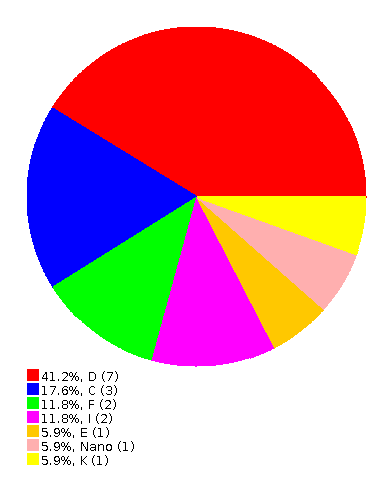
\includegraphics[scale=0.5]{../img/survey/pie.png}

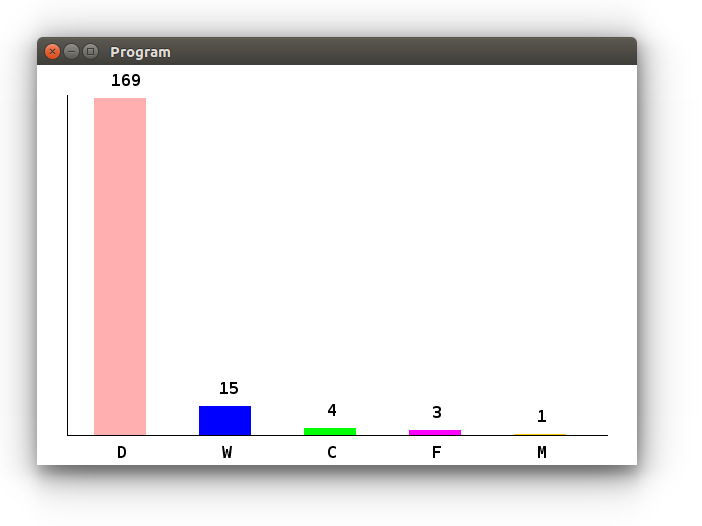
\includegraphics[scale=0.5]{../img/survey/bar.png}
